\documentclass{article}
\usepackage{amsthm}
\usepackage{amsmath}
\usepackage{amsfonts}
\usepackage{tikz}
\usepackage{amssymb}

\newtheorem*{definition}{Definição}
\newtheorem*{theorem}{Teorema}
\newtheorem*{exemple}{Exemplo}
\newtheorem*{atencao}{Atenção}
\newtheorem*{proposicao}{Proposição}
\newtheorem*{ex}{Exercício}
\usepackage{mathtools}
\usepackage{xfrac}
\DeclarePairedDelimiter\abs{\lvert}{\rvert}%
\DeclareMathOperator{\Ima}{Im}

\setlength{\textwidth}{450pt}
\setlength{\marginparwidth}{0pt}
\setlength{\marginparsep}{0pt}
\usepackage[left=2.5cm, right=2.5cm]{geometry}

\title{Trabalho 1 \\ \large Grupos e Corpos}
\author{Yuri Kosfeld}
\date{Abril 2025}

\begin{document}

\maketitle

\begin{ex}[Semana 1 - 13]
    (a) Para facilitar a explicação, vamos numerar os vértices do poligono de maneira ordenada de 1 até n.
    Uma rotação nesse poligono é uma forma de ciclar entre os vértices. Então se o nosso poligono
    tem 4 lados, temos 4 vértices: 1, 2, 3, 4. Se aplicarmos uma rotação nesse poligono os vértices
    agora trocam de indexação e vao de 1234 para 4123. Aplicando mais uma vez vamos para 3412 e assim por diante.
    A relação $r^n = 1$ é equivalente a dizer aplicar n rotações no poligono é a mesma ação de não aplicar rotação nenhuma.
    Visualmente é intuitivo pensar dessa forma, por exemplo, no nossa caso de n = 4, se olharmos
    o vértices da primeira posição, apos 4 rotações voltamos ao 1, ou seja, é igual a não ter feito
    rotação alguma. As reflexões no poligono são equivalentes a espelhamentos sobre um eixo do poligono de simetria desse poligono.
    Ou seja, as reflexões sobre um dado eixo não podem "mudar" o nosso poligono. De modo geral temos duas 
    possibilidades de reflexões, as que fixam vértices e as que não vixam vértice algum.
    Em ambos os casos não é dificil notar que aplicando a mesma reflexão duas vezes seguidas
    voltamos ao estado inicial. Assim vem a relação de $s^2=1$.
    \begin{center}
        \tikzset{every picture/.style={line width=0.75pt}} %set default line width to 0.75pt       
        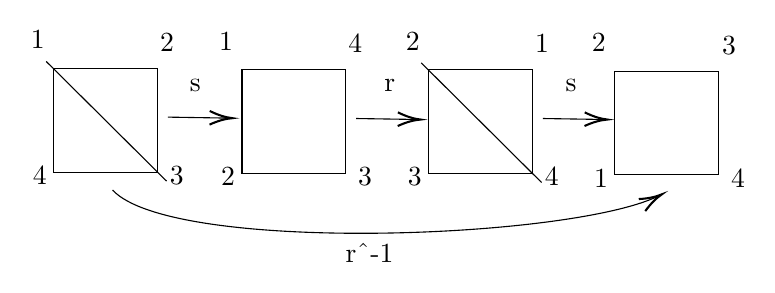
\begin{tikzpicture}[x=0.75pt,y=0.75pt,yscale=-1,xscale=1]
        %uncomment if require: \path (0,300); %set diagram left start at 0, and has height of 300

        %Shape: Square [id:dp11542187000741944] 
        \draw   (50,60) -- (100,60) -- (100,110) -- (50,110) -- cycle ;
        %Straight Lines [id:da31369456332723833] 
        \draw    (105,83.5) -- (134,83.97) ;
        \draw [shift={(136,84)}, rotate = 180.92] [color={rgb, 255:red, 0; green, 0; blue, 0 }  ][line width=0.75]    (10.93,-3.29) .. controls (6.95,-1.4) and (3.31,-0.3) .. (0,0) .. controls (3.31,0.3) and (6.95,1.4) .. (10.93,3.29)   ;
        %Straight Lines [id:da31002343470221183] 
        \draw    (46.33,56.67) -- (104.33,114.33) ;
        %Shape: Square [id:dp9946696417593814] 
        \draw   (140.67,60.67) -- (190.67,60.67) -- (190.67,110.67) -- (140.67,110.67) -- cycle ;
        %Straight Lines [id:da6966810167833951] 
        \draw    (195.67,84.17) -- (224.67,84.63) ;
        \draw [shift={(226.67,84.67)}, rotate = 180.92] [color={rgb, 255:red, 0; green, 0; blue, 0 }  ][line width=0.75]    (10.93,-3.29) .. controls (6.95,-1.4) and (3.31,-0.3) .. (0,0) .. controls (3.31,0.3) and (6.95,1.4) .. (10.93,3.29)   ;
        %Shape: Square [id:dp5694789197294783] 
        \draw   (230.67,60.67) -- (280.67,60.67) -- (280.67,110.67) -- (230.67,110.67) -- cycle ;
        %Straight Lines [id:da49098578373547497] 
        \draw    (285.67,84.17) -- (314.67,84.63) ;
        \draw [shift={(316.67,84.67)}, rotate = 180.92] [color={rgb, 255:red, 0; green, 0; blue, 0 }  ][line width=0.75]    (10.93,-3.29) .. controls (6.95,-1.4) and (3.31,-0.3) .. (0,0) .. controls (3.31,0.3) and (6.95,1.4) .. (10.93,3.29)   ;
        %Straight Lines [id:da29576404756363095] 
        \draw    (227,57.33) -- (285,115) ;
        %Shape: Square [id:dp8601576122979447] 
        \draw   (320.33,61.33) -- (370.33,61.33) -- (370.33,111.33) -- (320.33,111.33) -- cycle ;
        %Curve Lines [id:da18440816847451147] 
        \draw    (78.33,118.67) .. controls (107.04,149.36) and (299.1,142.48) .. (341.75,121.31) ;
        \draw [shift={(343,120.67)}, rotate = 151.56] [color={rgb, 255:red, 0; green, 0; blue, 0 }  ][line width=0.75]    (10.93,-3.29) .. controls (6.95,-1.4) and (3.31,-0.3) .. (0,0) .. controls (3.31,0.3) and (6.95,1.4) .. (10.93,3.29)   ;

        % Text Node
        \draw (37.67,40.67) node [anchor=north west][inner sep=0.75pt]   [align=left] {1};
        % Text Node
        \draw (100,42) node [anchor=north west][inner sep=0.75pt]   [align=left] {2};
        % Text Node
        \draw (104.67,106) node [anchor=north west][inner sep=0.75pt]   [align=left] {3};
        % Text Node
        \draw (38.67,106) node [anchor=north west][inner sep=0.75pt]   [align=left] {4};
        % Text Node
        \draw (128.33,41.33) node [anchor=north west][inner sep=0.75pt]   [align=left] {1};
        % Text Node
        \draw (190.67,42.67) node [anchor=north west][inner sep=0.75pt]   [align=left] {4};
        % Text Node
        \draw (195.33,106.67) node [anchor=north west][inner sep=0.75pt]   [align=left] {3};
        % Text Node
        \draw (129.33,106.67) node [anchor=north west][inner sep=0.75pt]   [align=left] {2};
        % Text Node
        \draw (218.33,41.33) node [anchor=north west][inner sep=0.75pt]   [align=left] {2};
        % Text Node
        \draw (280.67,42.67) node [anchor=north west][inner sep=0.75pt]   [align=left] {1};
        % Text Node
        \draw (285.33,106.67) node [anchor=north west][inner sep=0.75pt]   [align=left] {4};
        % Text Node
        \draw (219.33,106.67) node [anchor=north west][inner sep=0.75pt]   [align=left] {3};
        % Text Node
        \draw (308,42) node [anchor=north west][inner sep=0.75pt]   [align=left] {2};
        % Text Node
        \draw (370.67,43.33) node [anchor=north west][inner sep=0.75pt]   [align=left] {3};
        % Text Node
        \draw (375,107.33) node [anchor=north west][inner sep=0.75pt]   [align=left] {4};
        % Text Node
        \draw (309,107.33) node [anchor=north west][inner sep=0.75pt]   [align=left] {1};
        % Text Node
        \draw (114.33,64.33) node [anchor=north west][inner sep=0.75pt]   [align=left] {s};
        % Text Node
        \draw (295.33,64) node [anchor=north west][inner sep=0.75pt]   [align=left] {s};
        % Text Node
        \draw (208,64) node [anchor=north west][inner sep=0.75pt]   [align=left] {r};
        % Text Node
        \draw (189.33,143) node [anchor=north west][inner sep=0.75pt]   [align=left] {r\textasciicircum -1};
        \end{tikzpicture}
    \end{center}
    (b) Como $D_n$ é gerado por todos os possiveis produtos de rotações e reflexões, para calcular
    a ordem de $D_n$ é suficiente contar quantas rotações e quantas reflexões são possiveis a depender de n.
    Pela relação $r^n = 1$ segue que temos n rotações em $D_n$. Agora para as reflexões, precisamos
    separar nos casos, n par e n impar. Se n for par, então temos dois tipos de reflexões, as que fixam 
    dois vértices e as que não vixam nenhum. Para as que fixam 2 vértices, temos então $n/2$ reflexões possiveis.
    Já para as reflexões que não fixam nenhum vértice, elas são as reflexões cujos eixos passam pelos
    pontos medios de lados opostos. Assim também temos $n/2$ reflexões. Logo o número total de reflexões é n.
    Para n impar, é mais simples. As únicas reflexões são aquelas que fixam um vértice, logo 
    temos n reflexões. Assim
    \[|D_n| = |\text{rotações}| + |\text{reflexões}| = n + n = 2n\]
    (c)
    \begin{center}
        \tikzset{every picture/.style={line width=0.75pt}} %set default line width to 0.75pt        

        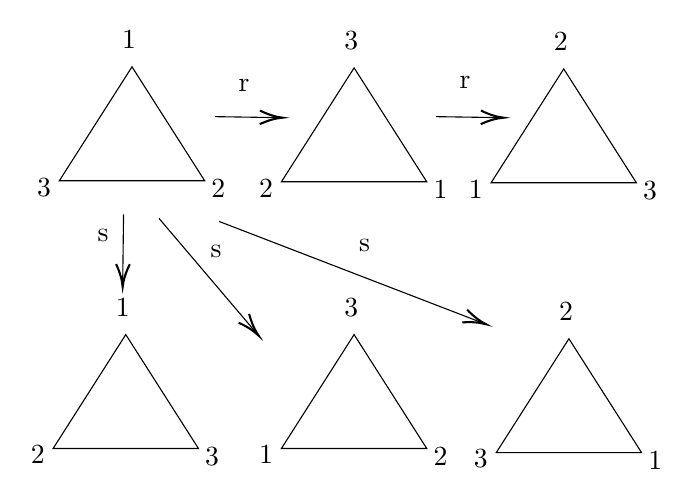
\begin{tikzpicture}[x=0.75pt,y=0.75pt,yscale=-1,xscale=1]
        %uncomment if require: \path (0,253); %set diagram left start at 0, and has height of 253

        %Shape: Triangle [id:dp27316798163488343] 
        \draw   (217.5,32.5) -- (252.5,87.36) -- (182.5,87.36) -- cycle ;
        %Shape: Triangle [id:dp5149210388591837] 
        \draw   (324.5,33) -- (359.5,87.86) -- (289.5,87.86) -- cycle ;
        %Shape: Triangle [id:dp06578896516364685] 
        \draw   (425.5,33.5) -- (460.5,88.36) -- (390.5,88.36) -- cycle ;
        %Shape: Triangle [id:dp4198540414173709] 
        \draw   (214.5,161.5) -- (249.5,216.36) -- (179.5,216.36) -- cycle ;
        %Shape: Triangle [id:dp908594080810223] 
        \draw   (324.5,161.5) -- (359.5,216.36) -- (289.5,216.36) -- cycle ;
        %Shape: Triangle [id:dp2676478360786132] 
        \draw   (428,163.5) -- (463,218.36) -- (393,218.36) -- cycle ;
        %Straight Lines [id:da09562310036490274] 
        \draw    (257.5,56.5) -- (288,56.97) ;
        \draw [shift={(290,57)}, rotate = 180.88] [color={rgb, 255:red, 0; green, 0; blue, 0 }  ][line width=0.75]    (10.93,-3.29) .. controls (6.95,-1.4) and (3.31,-0.3) .. (0,0) .. controls (3.31,0.3) and (6.95,1.4) .. (10.93,3.29)   ;
        %Straight Lines [id:da2805382139907] 
        \draw    (364,56.5) -- (394.5,56.97) ;
        \draw [shift={(396.5,57)}, rotate = 180.88] [color={rgb, 255:red, 0; green, 0; blue, 0 }  ][line width=0.75]    (10.93,-3.29) .. controls (6.95,-1.4) and (3.31,-0.3) .. (0,0) .. controls (3.31,0.3) and (6.95,1.4) .. (10.93,3.29)   ;
        %Straight Lines [id:da36402917029534343] 
        \draw    (213.43,103.58) -- (213.02,136.5) ;
        \draw [shift={(213,138.5)}, rotate = 270.7] [color={rgb, 255:red, 0; green, 0; blue, 0 }  ][line width=0.75]    (10.93,-3.29) .. controls (6.95,-1.4) and (3.31,-0.3) .. (0,0) .. controls (3.31,0.3) and (6.95,1.4) .. (10.93,3.29)   ;
        %Straight Lines [id:da4144241143801658] 
        \draw    (230.5,105.5) -- (277.21,160.48) ;
        \draw [shift={(278.5,162)}, rotate = 229.65] [color={rgb, 255:red, 0; green, 0; blue, 0 }  ][line width=0.75]    (10.93,-3.29) .. controls (6.95,-1.4) and (3.31,-0.3) .. (0,0) .. controls (3.31,0.3) and (6.95,1.4) .. (10.93,3.29)   ;
        %Straight Lines [id:da6082468836407046] 
        \draw    (259.5,107) -- (386.13,155.78) ;
        \draw [shift={(388,156.5)}, rotate = 201.07] [color={rgb, 255:red, 0; green, 0; blue, 0 }  ][line width=0.75]    (10.93,-3.29) .. controls (6.95,-1.4) and (3.31,-0.3) .. (0,0) .. controls (3.31,0.3) and (6.95,1.4) .. (10.93,3.29)   ;

        % Text Node
        \draw (211.5,13.9) node [anchor=north west][inner sep=0.75pt]    {$1$};
        % Text Node
        \draw (170.5,84.9) node [anchor=north west][inner sep=0.75pt]    {$3$};
        % Text Node
        \draw (254.5,85.76) node [anchor=north west][inner sep=0.75pt]    {$2$};
        % Text Node
        \draw (318.5,14.4) node [anchor=north west][inner sep=0.75pt]    {$3$};
        % Text Node
        \draw (277.5,85.4) node [anchor=north west][inner sep=0.75pt]    {$2$};
        % Text Node
        \draw (361.5,86.26) node [anchor=north west][inner sep=0.75pt]    {$1$};
        % Text Node
        \draw (419.5,14.9) node [anchor=north west][inner sep=0.75pt]    {$2$};
        % Text Node
        \draw (378.5,85.9) node [anchor=north west][inner sep=0.75pt]    {$1$};
        % Text Node
        \draw (462.5,86.76) node [anchor=north west][inner sep=0.75pt]    {$3$};
        % Text Node
        \draw (208.5,142.9) node [anchor=north west][inner sep=0.75pt]    {$1$};
        % Text Node
        \draw (167.5,213.9) node [anchor=north west][inner sep=0.75pt]    {$2$};
        % Text Node
        \draw (251.5,214.76) node [anchor=north west][inner sep=0.75pt]    {$3$};
        % Text Node
        \draw (318.5,142.9) node [anchor=north west][inner sep=0.75pt]    {$3$};
        % Text Node
        \draw (277.5,213.9) node [anchor=north west][inner sep=0.75pt]    {$1$};
        % Text Node
        \draw (361.5,214.76) node [anchor=north west][inner sep=0.75pt]    {$2$};
        % Text Node
        \draw (422,144.9) node [anchor=north west][inner sep=0.75pt]    {$2$};
        % Text Node
        \draw (381,215.9) node [anchor=north west][inner sep=0.75pt]    {$3$};
        % Text Node
        \draw (465,216.76) node [anchor=north west][inner sep=0.75pt]    {$1$};
        % Text Node
        \draw (267.64,37.5) node [anchor=north west][inner sep=0.75pt]   [align=left] {r};
        % Text Node
        \draw (374.14,36) node [anchor=north west][inner sep=0.75pt]   [align=left] {r};
        % Text Node
        \draw (199.64,109.5) node [anchor=north west][inner sep=0.75pt]   [align=left] {s};
        % Text Node
        \draw (254.14,117.5) node [anchor=north west][inner sep=0.75pt]   [align=left] {s};
        % Text Node
        \draw (325.64,114.5) node [anchor=north west][inner sep=0.75pt]   [align=left] {s};
        \end{tikzpicture}
    \end{center}
    \begin{center}
        $D_3$
    \end{center}
    \begin{center}
        \tikzset{every picture/.style={line width=0.75pt}} %set default line width to 0.75pt        

        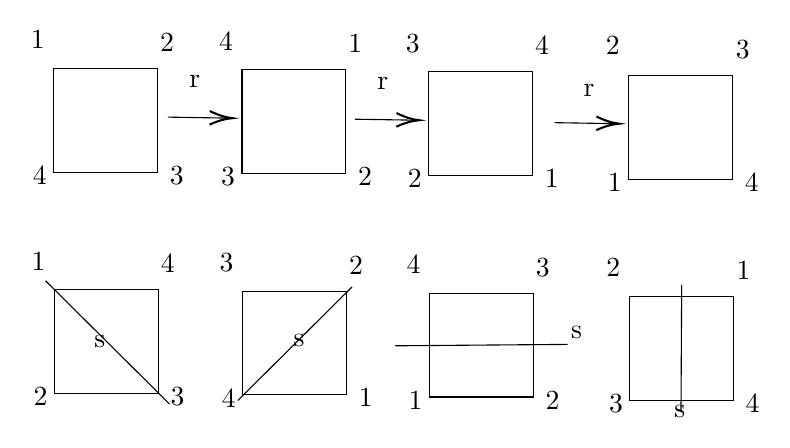
\begin{tikzpicture}[x=0.75pt,y=0.75pt,yscale=-1,xscale=1]
        %uncomment if require: \path (0,300); %set diagram left start at 0, and has height of 300

        %Shape: Square [id:dp7216412607374494] 
        \draw   (31,35.33) -- (81,35.33) -- (81,85.33) -- (31,85.33) -- cycle ;
        %Straight Lines [id:da018946078414078027] 
        \draw    (86,58.83) -- (115,59.3) ;
        \draw [shift={(117,59.33)}, rotate = 180.92] [color={rgb, 255:red, 0; green, 0; blue, 0 }  ][line width=0.75]    (10.93,-3.29) .. controls (6.95,-1.4) and (3.31,-0.3) .. (0,0) .. controls (3.31,0.3) and (6.95,1.4) .. (10.93,3.29)   ;
        %Shape: Square [id:dp3211094666869254] 
        \draw   (121.67,36) -- (171.67,36) -- (171.67,86) -- (121.67,86) -- cycle ;
        %Straight Lines [id:da18400820847151056] 
        \draw    (176,59.83) -- (205,60.3) ;
        \draw [shift={(207,60.33)}, rotate = 180.92] [color={rgb, 255:red, 0; green, 0; blue, 0 }  ][line width=0.75]    (10.93,-3.29) .. controls (6.95,-1.4) and (3.31,-0.3) .. (0,0) .. controls (3.31,0.3) and (6.95,1.4) .. (10.93,3.29)   ;
        %Shape: Square [id:dp597588242882821] 
        \draw   (211.67,37) -- (261.67,37) -- (261.67,87) -- (211.67,87) -- cycle ;
        %Straight Lines [id:da6641535414657286] 
        \draw    (272.33,61.5) -- (301.33,61.97) ;
        \draw [shift={(303.33,62)}, rotate = 180.92] [color={rgb, 255:red, 0; green, 0; blue, 0 }  ][line width=0.75]    (10.93,-3.29) .. controls (6.95,-1.4) and (3.31,-0.3) .. (0,0) .. controls (3.31,0.3) and (6.95,1.4) .. (10.93,3.29)   ;
        %Shape: Square [id:dp04533339988683438] 
        \draw   (308,38.67) -- (358,38.67) -- (358,88.67) -- (308,88.67) -- cycle ;
        %Shape: Square [id:dp21519751857132374] 
        \draw   (31.33,142) -- (81.33,142) -- (81.33,192) -- (31.33,192) -- cycle ;
        %Shape: Square [id:dp9433827211127012] 
        \draw   (122,142.67) -- (172,142.67) -- (172,192.67) -- (122,192.67) -- cycle ;
        %Shape: Square [id:dp09312841383495163] 
        \draw   (212,143.67) -- (262,143.67) -- (262,193.67) -- (212,193.67) -- cycle ;
        %Shape: Square [id:dp7986970731534507] 
        \draw   (308.33,145.33) -- (358.33,145.33) -- (358.33,195.33) -- (308.33,195.33) -- cycle ;
        %Straight Lines [id:da48326344257362375] 
        \draw    (27,137.67) -- (86.67,197) ;
        %Straight Lines [id:da9632376599339169] 
        \draw    (119.67,195.33) -- (174.67,140.67) ;
        %Straight Lines [id:da801522782031135] 
        \draw    (195.5,169) -- (278.5,168.33) ;
        %Straight Lines [id:da39167069544145217] 
        \draw    (333.17,201) -- (333.5,139.67) ;

        % Text Node
        \draw (18.67,16) node [anchor=north west][inner sep=0.75pt]   [align=left] {1};
        % Text Node
        \draw (81,17.33) node [anchor=north west][inner sep=0.75pt]   [align=left] {2};
        % Text Node
        \draw (85.67,81.33) node [anchor=north west][inner sep=0.75pt]   [align=left] {3};
        % Text Node
        \draw (19.67,81.33) node [anchor=north west][inner sep=0.75pt]   [align=left] {4};
        % Text Node
        \draw (109.33,16.67) node [anchor=north west][inner sep=0.75pt]   [align=left] {4};
        % Text Node
        \draw (171.67,18) node [anchor=north west][inner sep=0.75pt]   [align=left] {1};
        % Text Node
        \draw (176.33,82) node [anchor=north west][inner sep=0.75pt]   [align=left] {2};
        % Text Node
        \draw (110.33,82) node [anchor=north west][inner sep=0.75pt]   [align=left] {3};
        % Text Node
        \draw (199.33,17.67) node [anchor=north west][inner sep=0.75pt]   [align=left] {3};
        % Text Node
        \draw (261.67,19) node [anchor=north west][inner sep=0.75pt]   [align=left] {4};
        % Text Node
        \draw (266.33,83) node [anchor=north west][inner sep=0.75pt]   [align=left] {1};
        % Text Node
        \draw (200.33,83) node [anchor=north west][inner sep=0.75pt]   [align=left] {2};
        % Text Node
        \draw (295.67,19) node [anchor=north west][inner sep=0.75pt]   [align=left] {2};
        % Text Node
        \draw (358.33,20.67) node [anchor=north west][inner sep=0.75pt]   [align=left] {3};
        % Text Node
        \draw (362.67,84.67) node [anchor=north west][inner sep=0.75pt]   [align=left] {4};
        % Text Node
        \draw (296.67,84.67) node [anchor=north west][inner sep=0.75pt]   [align=left] {1};
        % Text Node
        \draw (95,37.67) node [anchor=north west][inner sep=0.75pt]   [align=left] {r};
        % Text Node
        \draw (185.67,38.33) node [anchor=north west][inner sep=0.75pt]   [align=left] {r};
        % Text Node
        \draw (285,41.67) node [anchor=north west][inner sep=0.75pt]   [align=left] {r};
        % Text Node
        \draw (19,122.67) node [anchor=north west][inner sep=0.75pt]   [align=left] {1};
        % Text Node
        \draw (81.33,124) node [anchor=north west][inner sep=0.75pt]   [align=left] {4};
        % Text Node
        \draw (86,188) node [anchor=north west][inner sep=0.75pt]   [align=left] {3};
        % Text Node
        \draw (20,188) node [anchor=north west][inner sep=0.75pt]   [align=left] {2};
        % Text Node
        \draw (109.67,123.33) node [anchor=north west][inner sep=0.75pt]   [align=left] {3};
        % Text Node
        \draw (172,124.67) node [anchor=north west][inner sep=0.75pt]   [align=left] {2};
        % Text Node
        \draw (176.67,188.33) node [anchor=north west][inner sep=0.75pt]   [align=left] {1};
        % Text Node
        \draw (110.67,188.67) node [anchor=north west][inner sep=0.75pt]   [align=left] {4};
        % Text Node
        \draw (199.67,124.33) node [anchor=north west][inner sep=0.75pt]   [align=left] {4};
        % Text Node
        \draw (262,125.67) node [anchor=north west][inner sep=0.75pt]   [align=left] {3};
        % Text Node
        \draw (266.67,189.67) node [anchor=north west][inner sep=0.75pt]   [align=left] {2};
        % Text Node
        \draw (200.67,189.67) node [anchor=north west][inner sep=0.75pt]   [align=left] {1};
        % Text Node
        \draw (296,125.67) node [anchor=north west][inner sep=0.75pt]   [align=left] {2};
        % Text Node
        \draw (358.67,127) node [anchor=north west][inner sep=0.75pt]   [align=left] {1};
        % Text Node
        \draw (363,191.33) node [anchor=north west][inner sep=0.75pt]   [align=left] {4};
        % Text Node
        \draw (297.33,191.33) node [anchor=north west][inner sep=0.75pt]   [align=left] {3};
        % Text Node
        \draw (49.33,162.67) node [anchor=north west][inner sep=0.75pt]   [align=left] {s};
        % Text Node
        \draw (279,158.33) node [anchor=north west][inner sep=0.75pt]   [align=left] {s};
        % Text Node
        \draw (145.33,162.33) node [anchor=north west][inner sep=0.75pt]   [align=left] {s};
        % Text Node
        \draw (328.67,196.67) node [anchor=north west][inner sep=0.75pt]   [align=left] {s};
        \end{tikzpicture}
    \end{center}
    \begin{center}
        $D_4$
    \end{center}
    (d) Para $D_4$ ser ciclico, ele deve ser gerado por um único elemento de $D_4$.
    Vamos mostrar que isso não é possivel.
    Tome primeiro r uma rotação. Pela relação $r^n = 1$, temos que $\left\langle r\right\rangle = \{1, r, r^2, r^3\}$,
    e então faltam as reflexões. Tome então uma s uma reflexão de $D_4$.
    Novamente pela relação $s^2=1$, temos que $\left\langle s\right\rangle = \{1, s\}$, assim faltando todas as demais reflexões e todas as rotações.
    Logo nenhum elemento de $D_4$ gera todo as simetrias e portanto $D_4$ não é ciclico.
    (e) Antes de mostrarmos que $D_n < S_n$, vamos ver que toda simetria em $D_n$ é uma permutação dos vértices.
    Para isso, vamos mostrar que rotações e reflexões são permutação, e como esses são os geradores das simetrias 
    em $D_n$, mostramos que todas são.
    Uma rotação em um poligono de n lados é uma permutação ciclica nos vertices do poligono. 
    Então r uma rotação leva $r(i)=i+1$. Por exemplo, em $D_4$, uma rotação 
    de $90^{\circ}$ no sentido horário é a permutação dos vértices $(1234)$.
    Já uma reflexão é uma permutação que age nos vertices em pares. Note 
    que em ambos os casos de reflexão isso vale, já que uma reflexão que fixa
    um vertice (caso n ímpar), temos $n-1$ vértices para mudar e como n é impar, n-1 é par, logo temos $\frac{n-1}{2}$ mudanças.
    Para o caso n par, isso também vale, seja fixando um par de vértices ou não fixando nenhum.
    Como as simetrias são geradas por rotações e reflexões, qualquer produto de duas simetrias ainda é uma simetria em $D_n$, logo é fechado para o produto.
    Temos também um elemento neutro, a simetria identidade.
    Além disso, toda simetria tem um elemento inverso. Para mostrar isso vamos mostrar que toda rotação e toda reflexão possuem inversos.
    Tome $r_k$ uma rotação, sabemos que vale a relação $r^n=1$, então se r é uma rotação dada por
    $r_k(i)=i+k$, segue que $r_k = r^k$ e então o inverso de $r_k$ é $r^{n-k}$, 
    uma vez que, $r_kr^{n-k}=r^kr^{n-k}=r^{n-k+k}=r^n=1$. Para as reflexões, basta notar que
    segue da relação $s^2=1$ que o inverso é ela mesma.
    Assim $D_n$ é um subgrupo de $S_n$.
\end{ex}

\begin{ex}[Semana 2 - 4]
    Primeiro precisamo mostrar que $G/G'$ é um grupo. 
    Para isso, basta verificar se $G' \vartriangleleft G$.
    Tome então um comutador de G, ou seja, $[x, y] \in G'$ e vamos mostrar que vale a inclusão para todo $g \in G$.
    Lembre que vale $[x, y]= xyx^{-1}y^{-1}$, então segue
    \[g[x,y]g^{-1}=g(xyx^{-1}y^{-1})g^{-1}=(gxg^{-1})(gyg^{-1})(gx^{-1}g^{-1})(gy^{-1}g^{-1})\]
    Vamos mostrar que $(gxg^{-1})^{-1}=gx^{-1}g^{-1}$. Seja então d o inverso de $gxg^{-1}$, segue então
    \begin{align*}
        gxg^{-1}d &= 1 \\
        xg^{-1}d &= g^{-1} \\
        g^{-1}d &= x^{-1}g^{-1} \\
        d &= gx^{-1}g^{-1}
    \end{align*}
    Note que o mesmo vale para y.
    Então temos que 
    \[g[x,y]g^{-1} = (gxg^{-1})(gyg^{-1})(gxg^{-1})^{-1}(gyg^{-1})^{-1}=[gxg^{-1}, gyg^{-1}] \in G'\]
    Logo $G' \vartriangleleft G$.
    Agora que garantimos que $G/G'$ é um grupo, vamos mostrar que ele é abeliano. 
    Queremos mostrar então para $g_1, g_2 \in G$
    \[(g_1G')(g_2G') = (g_2G')(g_1G') \Leftrightarrow g_1g_2G'=g_2g_2G'\]
    Ou seja, queremos ver ser $g_1g_2(g_2g_1)^{-1} \in G'$. 
    Mas note que, $g_1g_2(g_2g_1)^{-1} = g_1g_2g_2^{-1}g_1^{-1} = [g_1, g_2] \in G'$.
    Logo $G/G'$ é abeliano.
\end{ex}

\begin{ex}[Semana 2 - 11]
    Primeiro vamos notar o que acontece com 
\end{ex}

\begin{ex}[Semana 2 - 12]
    Queremos mostrar que existe $x \in G$ tal que a ordem de x é p.
    Para isso vamos provar usando indução na ordem de G. Denotaremos $|G|= n $.
    Como caso base, vamos verificar quando $n = p$.
    Segue pelo corolario do Teorema de Lagrange, que G é ciclico, logo $G = \left\langle x \right\rangle $, 
    e portanto $o(x) = |G|$, equivalente a $x^p = e_G$. Assim provado para o caso base.
    Lembre que G é abeliano. Tome então $a \in G$ tal que $a \neq e_G$ e defina $H = \left\langle a \right\rangle $.
    Se $p \vert |H|$ então $a^{|H|/p}$ é um elemento de ordem p, e novamente temos solução.
    Se $p \nmid |H|$ então pelo Teorema de Lagrange, $p \vert (G : H)$.
    Mas $(G : H) = |G / H|$ e portanto $p \vert | G / H|$.
    Logo pela hipotese de indução, tem um elemento de $xH$ para algum $x \in G$ que tem ordem p.
    Seja m é a ordem de x em G, então $(xH)^m=eH \in G/H$. 
    Donde segue que $p\vert m$ e então $x^{m/p}$ tem ordem p.
\end{ex}

\begin{ex}[Semana 3 - 7]
    Queremos mostrar que $Z(G)$ não é trivial.
    Para isso, vamos provar que \[|Z(G)| > 1\] já que se $Z(G)$ fosse trivial, teriamos $Z(G) = \{e_G\}$ e então $|Z(G)| = 1$.
    Sabemos que a ordem de G é uma potência de p, então p divide a ordem de G.
    Então pela Equação das Classes Conjugadas de G, todos os termos $(G:C(g_i))$ são diviseis por p.
    Pelo Teorema de Lagrange, $(G:C(g_i))$ é um divisor da ordem de G e portanto é uma potência de p. 
    Novamente, pela Equação das Classes Conjugadas de G, temos 
    \[ p^n = | G | = | Z(G) | + \sum p^m_i\]
    em que cada $m_i$ é o expoente de cada $(G:C(g_i))$.
    Logo,
    \[| Z(G) | \equiv p^n - \sum p^m_i \equiv 0 \mod p\]
    Como $| Z(G) | \geq 1$ e $| Z(G) | \equiv 0 \mod p$ temos que $| Z(G) | \geq p > 1$.
    Assim $Z(G)$ é não trivial.
\end{ex}

\begin{ex}[Semana 3 - 8]
    Para provarmos esse resultado, primeiro vamos notar primeiro que G é abeliano se somente se $G = Z(G)$.
    Não é dificl notar isso dado a definição do centro de G.
    Dadas as hipoteses de G, vamos mostrar que G é abeliano.
    Suponha por contradição que $Z(G) \neq G$. 
    Tome então $a \in G \setminus Z(G)$.
    Assim $C(a)$ é subgrupo de G que contém a e Z(G), já que todos os elementos de Z(G) comutam.
    Como vimos no exercicio anterior, Z(G) não é trivial e mais, $|Z(G)| \geq p$.
    Além disso, temos também que $|C(a)| \geq |Z(G)| + 1 = p + 1$.
    Pelo Teorema de Lagrange, a ordem de C(a) deve dividir a ordem de G.
    Logo temos duas, possibilidades: ou $|C(a)| = p$ ou $|C(a)|=p^2$. 
    Mas como visto anteriormente, $|C(a)| \geq p + 1$ assim a única possibilidade válida é $|C(a)| = p^2$.
    Então $C(a) = G$ e então todos os elementos de G comutam e portanto $a \in Z(G)$ uma contradição.
\end{ex}

\begin{ex}[Semana 3 - 12]
    Vamos analisar os p-subgupos de Sylow para G.
    Segue do Terceiro Teorema de Sylow que $n_q \equiv 1 \mod q$ e $n_q \vert p$.
    Temos então duas possibilidades para $n_q$.
    Se $n_q = p$ então $p \equiv 1 \mod q$, o que não pode acontecer, já que $p < q$ e são primos.
    Logo, por força $n_q = 1$. Ou seja, existe um unico q-subgrupo de sylow. 
    Seja Q esse subgrupo, e então sabemos que Q é normal pela unicidade.
    Vamos analisar agora $n_p$. 
    $n_p \equiv 1 \mod p$ e $n_p \vert q$.
    Nessas condições, vamos ver que $n_p = 1$ ou $n_p = q$.
    Se $n_p = q$ então $q - 1 \equiv 0 \mod p$, o que contradiz a hipotese de $p \nmid q-1$.
    Logo $n_p =1 $ e também tem um unico P p-sugrupo de sylow em G e portanto P é normal.
    Sabemos que $P \cap Q = \{e_G\}$.
    Queremos mostrar agora que $PQ = QP$, ou seja, que PQ é abeliano.
    Para todo $x \in P$ e $y \in Q$ considere $xyx^{-1}y^{-1}$.
    Como Q é normal, segue que $xyx^{-1} \in Q \Rightarrow xyx^{-1}y^{-1} \in Q$.
    Também temos que P é normal, portanto $yxy^{-1} \in P \Rightarrow xyx^{-1}y^{-1} \in P$.
    Mas como vimos pela interseção de P e Q, segue então $xyx^{-1}y^{-1} = 1 \Rightarrow xy = yx$.
    Finalmente, temos que $|PQ| = pq = |G|$ e então $G = PQ$ e G é abeliano.
\end{ex}

\begin{ex}[Semana 4 - 6]
    Sabemos que em $S_4$ os únicos subgrupos normais são $\{e\}, V_4, A_4$ e o proprio $S_4$.
    Aqui $V_4$ é o grupo de Klein, dado por
    \[V_4 = \{ e, (12)(34), (13)(24), (14)(23) \}\]
    Sabemos que $V_4$ é abeliano e portanto todo subgrupo dele é normal. 
    Se então construirmos a serie subnormal 
    \[\{e\} \leq \left\langle (12)(34)\right\rangle \leq V_4 \leq S_4 \] 
    satisfaz as condições, dadas as propriedades de $V_4$, mas tem o grupo $\left\langle (12)(34)\right\rangle$ não é normal em $S_4$.
    Logo é uma serie subnormal que não é normal.
\end{ex}

\begin{ex}[Semana 4 - 7]
    
\end{ex}

\begin{ex}[Semana 4 - 11]
    Para isso vamos dividir nossos casos com base nas ordens possiveis que satisfazem certas propriedades.
    \textbf{Caso 1}: $|G| = p$ com p primo. Nesse caso temos que G é ciclico e portanto ciclico.
    Como G é abeliano sabemos que G é soluvel. Para esse caso, a cardinalidade de G pode ser
    \[|G| = 2, 3, 5, 7, 13, 19, 23, 29, 31, 37, 41, 43, 47, 53, 59\]
    \textbf{Caso 2}: Se G é um p-subgrupo. Como mostramos no exercicio 8 da semana 3, Z(G) não é trivial e também mostramos
    que G é abeliano. Logo novamente G é soluvel.
    As cardinalidades que se encaixam nesse caso são as de potencias de primo.
    Logo as cardinalidades desse caso são
    \[|G| = 4, 8, 9 ,16, 25, 27, 32, 49\]
    \textbf{Caso 3}: $|G| = pq$ com p, q primos com  $p \vert q-1 $. 
    Segue do exercicio 12 da semana 3 que G é abeliano, logo soluvel.
    As cardinalidades desse caso são
    \[|G| = 6, 10, 14, 15, 21, 22, 26, 33, 34, 35, 38, 39, 46, 51, 55, 57, 58\]
    \textbf{Caso 4}: $|G| = p^2q$. A prova é semelhante ao caso pq. Chegamos a conclusão
    que G tem so um unico p-sugrupo de sylow, logo é normal em G, e portanto G é soluvel.
    As cardinalidades desse caso são:
    \[|G| = 12, 18, 20, 28, 44, 45, 50, 52\]
    Acabaram de certa forma os casos, e agora precisamos verificar as caridinalidades que faltam.
    \textbf{$|G| = 24$}: Vamos mostrar que $|G| = 24$ não é simples. $24 = 2^{3}3$. 
    Pelo Terceiro Teorema de Sylow, $n_2 = 1$ ou $n_2$. Se $n_2 =1$, então G não é simples e portanto é soluvel.
    Assuma então $n_2 = 3$ G agindo por conjugação em 2-subgrupo de sylow, conseguimos um homomorfismo $\varphi: G \to S_3$.
    Como $24 = |G|>|S_3| = 6 $, temos que o nucleo de $\varphi$ não é trivial e normal. 
    \textbf{$|G| = 36$}: Novamente por sylow, $n_3 = 1$ ou $n_3 = 4$. $n_3 = 1$ é de novo não simples. 
    Seja então $n_3 = 4$, e por uma ação por conjugação semelhante ao caso anterior e G não é simples e então soluvel.
    \textbf{$|G| = 40 = 2^3 5$}: $n_5 \equiv 1 \mod 5$ e $n_5 \vert 2^3$, então por força $n_5 = 1$. Então o 5-sugbrupo de sylow 
    é unico e G é normal e portanto soluvel.
    \textbf{$|G| = 48 = 2^4 3$}: Se $n_2 = 3$ ou $n_3=4$, então temos um homomorfismo com kernel não trivial se 
    agirmos G por conjugação em 2-subgrupo de sylow de G ou 3-subgrupo de sylow de G, respectivamente.
    \textbf{$|G| = 54 = 2 \cdot 3^3$}: $n_3 \equiv 1 \mod 3$ e $n_3 \vert 2$, logo $n_3 =1 $ e portanto o 3-sugbrupo é unico e normal.
    \textbf{$|G| = 56 = 2^3 \cdot 7$}: Se $n_2 = 1 $ ou $n_7 = 1 $. Então $n_7 = 8$ Cada 7-subgrupo de sylow tem 7 elementos e todos eles se 
    intersectam somente no elemento neutro, logo G tem $8(7-1)=48$ elementos distintos de ordem 7. Logo é normal e portanto soluvel.
\end{ex}

\end{document}